\documentclass[11pt]{article}
\usepackage[letterpaper,margin=.25in]{geometry}
\usepackage{amsmath,amssymb,booktabs,array,tabularx,xcolor,tikz,hyperref,embedfile,microtype}
\usetikzlibrary{trees}
\hypersetup{colorlinks=true,urlcolor=blue!55!black}
\pagestyle{empty}
\setlength{\parindent}{0pt}
\setlength{\parskip}{4pt}
\linespread{1.035}\selectfont
\definecolor{navy}{RGB}{25,54,86}
\definecolor{soft}{RGB}{244,247,250}
\tikzset{branch/.style={circle,draw=navy,line width=.6pt,inner sep=2pt},trueleaf/.style={circle,draw=navy,fill=navy,inner sep=2.1pt},falseleaf/.style={circle,draw=navy,fill=white,inner sep=1.8pt}}
\newcommand{\sectionbar}[1]{\vspace{3pt}{\color{navy}\bfseries #1}\par\vspace{2pt}\hrule\vspace{4pt}}
\begin{document}
\enlargethispage{.12in}

\embedfile[desc={A244594 exact certificate payload},mimetype=application/json]{certificate_payload.json}
{\color{navy}\LARGE\bfseries A244594 concise calculus certificate}\hfill{\small VERIFIED}\\[-1pt]
{\small Bradley Klee, \quad Mech.An.ika Sol (Open AI) \hfill July 31, 2026}

\sectionbar{Definition and first terms}
\(\displaystyle (4-1\,x)\,A(x)=3+A(x)^{3}\), with the origin-normalized solution.\\
{\footnotesize Normalization/grammar: \texttt{A(x)=1+(1)*T(x); T=x+1*x*T+3*T\textasciicircum{}2+1*T\textasciicircum{}3}.}\\
\(a(0),\ldots,a(7)=1,1,4,29,263,2672,29088,331749\).\\[2pt]
{\small Kernel used throughout: \(\displaystyle \rho(u)=u\,\dfrac{1-3\,u^{1}-1\,u^{2}}{1+1\,u}\), so \(x=\rho(T(x))\).}

\sectionbar{Typogeometry}
\begin{minipage}[t]{.235\textwidth}\centering 
\begin{tikzpicture}[level distance=9mm,level 1/.style={sibling distance=10mm},level 2/.style={sibling distance=6mm},scale=.82,transform shape] \node[trueleaf] (n0) {};\end{tikzpicture}\\[2pt]{\normalsize\texttt{1x1}}\end{minipage}\begin{minipage}[t]{.235\textwidth}\centering 
\begin{tikzpicture}[level distance=9mm,level 1/.style={sibling distance=10mm},level 2/.style={sibling distance=6mm},scale=.82,transform shape] \node[branch,fill=orange!24] (n0) {} child {node[trueleaf] (n1) {}} child {node[trueleaf] (n2) {}};\end{tikzpicture}\\[2pt]{\normalsize\texttt{\{1,1\}x4}}\end{minipage}\begin{minipage}[t]{.235\textwidth}\centering 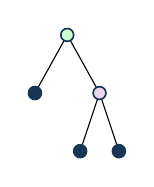
\begin{tikzpicture}[level distance=9mm,level 1/.style={sibling distance=10mm},level 2/.style={sibling distance=6mm},scale=.82,transform shape] \node[branch,fill=green!20] (n0) {} child {node[trueleaf] (n1) {}} child {node[branch,fill=violet!16] (n2) {} child {node[trueleaf] (n3) {}} child {node[trueleaf] (n4) {}}};\end{tikzpicture}\\[2pt]{\normalsize\texttt{\{1,\{1,1\}\}x16}}\end{minipage}\begin{minipage}[t]{.235\textwidth}\centering 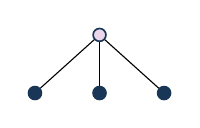
\begin{tikzpicture}[level distance=9mm,level 1/.style={sibling distance=10mm},level 2/.style={sibling distance=6mm},scale=.82,transform shape] \node[branch,fill=violet!16] (n0) {} child {node[trueleaf] (n1) {}} child {node[trueleaf] (n2) {}} child {node[trueleaf] (n3) {}};\end{tikzpicture}\\[2pt]{\normalsize\texttt{\{1,1,1\}x1}}\end{minipage}

{\footnotesize colored arity geometry; node color distinguishes constructors. Filled endpoints are true leaves; open endpoints are false/empty leaves. For colored grammars, color is genuine constructor data and is not silently converted into a positional zero pattern.}

{\footnotesize Typogeometric constructor codes and multiplicities: \(\Delta_{2}\!:\,3,\;\Delta_{2}^{\rm marked}\!:\,1,\;\Delta_{3}\!:\,1\).}

\sectionbar{Coefficient and contour extraction}
{\footnotesize \[\begin{gathered}\mathcal K_{n,h}=\{(k_1,\ldots,k_2)\in\mathbb Z_{\ge0}^{2}:h+\sum_{j=1}^{2}jk_j=n-1\},\quad K=\sum_{j=1}^{2}k_j,\\a(n)=\frac{1}{n}\sum_{h=0}^{n-1}\binom{n}{h}\sum_{\boldsymbol k\in\mathcal K_{n,h}}\binom{n+K-1}{K}\binom{K}{k_1,\ldots,k_2}3^{k_1}\,1^{k_2}.\end{gathered}\]}
\(a(n)=\dfrac{1}{2\pi i n}\oint_\gamma\dfrac{du}{\rho(u)^n},\quad n\ge1.\)

\sectionbar{Recurrence}
{\footnotesize \(\sum_{r=0}^{4}P_r(n)a(n+r)=0\), \(n\ge 1\), with \[\begin{aligned}P_{0}(n)&=4\,n^{3} + 2\,n^{2} - 2\,n\\P_{1}(n)&=-64\,n^{3} - 168\,n^{2} - 136\,n - 32\\P_{2}(n)&=384\,n^{3} + 1824\,n^{2} + 2848\,n + 1472\\P_{3}(n)&=-781\,n^{3} - 5825\,n^{2} - 14286\,n - 11520\\P_{4}(n)&=52\,n^{3} + 468\,n^{2} + 1352\,n + 1248\end{aligned}\]}

\sectionbar{Differential equation}
{\footnotesize \[\begin{aligned}&\left(0\right)A(x)+\left(4\,x^{5} - 32\,x^{4} + 64\,x^{3}\right)A'(x)\\[-1pt]&+\left(14\,x^{6} - 168\,x^{5} + 672\,x^{4} - 1139\,x^{3}\right)A^{(2)}(x)+\left(4\,x^{7} - 64\,x^{6} + 384\,x^{5} - 781\,x^{4} + 52\,x^{3}\right)A^{(3)}(x)=0.\end{aligned}\]}

\sectionbar{Matrices, telescoper certificate, and checks}
{\small \(\text{No compact matrix tuple is shown; see the embedded exact reduction data.}\)}
\par\vspace{6pt}
{\small\textbf{Certificate.}\par\smallskip\(\displaystyle R(n,u,x)=N/D\ \text{(exact }246\text{-character numerator in embedded payload)}.\)\par}
\vspace{4pt}
{\small Telescoping identity: \(\sum_r P_r(n)H_{n+r}(u)=\partial_u\!\left(R(n,u)H_n(u)\right).\)\par}
\vspace{4pt}
{\footnotesize Matrix dimensions: \(6\times 6\); remainder \(2\times 3\), rank 2, nullity 1. The exact telescoping residual is zero. The recurrence reconstructs all 24 stored terms; 6/6 published OEIS prefix terms match.\par}

\vfill
\colorbox{soft}{\parbox{.97\textwidth}{\tiny Canonical records: \texttt{data/tree\_model.json}, \texttt{data/contour.json}, \texttt{data/matrices.json}, \texttt{data/recurrence.json}, \texttt{data/ode.json}. Embedded payload contains exact sources and SHA-256 matrix identifiers. Compare with the verbose certificate for A120590.}}
\end{document}
